\newif\ifanswer\answertrue
%\answerfalse
\answertrue

\documentclass[10pt,dvipdfmx]{jsarticle}
\usepackage[margin=15truemm]{geometry}
\usepackage[dvipdfmx]{graphicx}
\usepackage{wrapfig}
\usepackage[dvipdfmx]{color}
\usepackage{ascmac} % for scree
\usepackage{subfigure} % for subfigure
\usepackage{multicol}
\usepackage{setspace}
\usepackage{diagbox}
\usepackage{fancyhdr}
\usepackage{xcolor}
\usepackage{here}
\usepackage{amsmath}
\usepackage{amssymb}
\usepackage{tikz}
\usetikzlibrary{intersections, calc, arrows.meta}
\usetikzlibrary{angles}
\usepackage{mathcomp}
\pagestyle{fancy}
\ifanswer
\lhead{理科まとめ 解答}
\else
\lhead{理科まとめ}
\fi
\rhead{\number\month\number\day}

\ifanswer
\newcommand{\answer}[2]{{\color{orange}#2}}
\newcommand{\page}[2]{#1}
\newcommand{\question}[2]{{\color{orange}#2}}
\else
\newcommand{\answer}[2]{\vspace{#1mm}}
\newcommand{\page}[2]{#2}
\newcommand{\question}[2]{#1}
\fi%answer


\begin{document}
\section{1年の生物}
\begin{itembox}[l]{植物の分類、分類基準も書け、分類は6種類}
	\answer{80}{
		\centering
		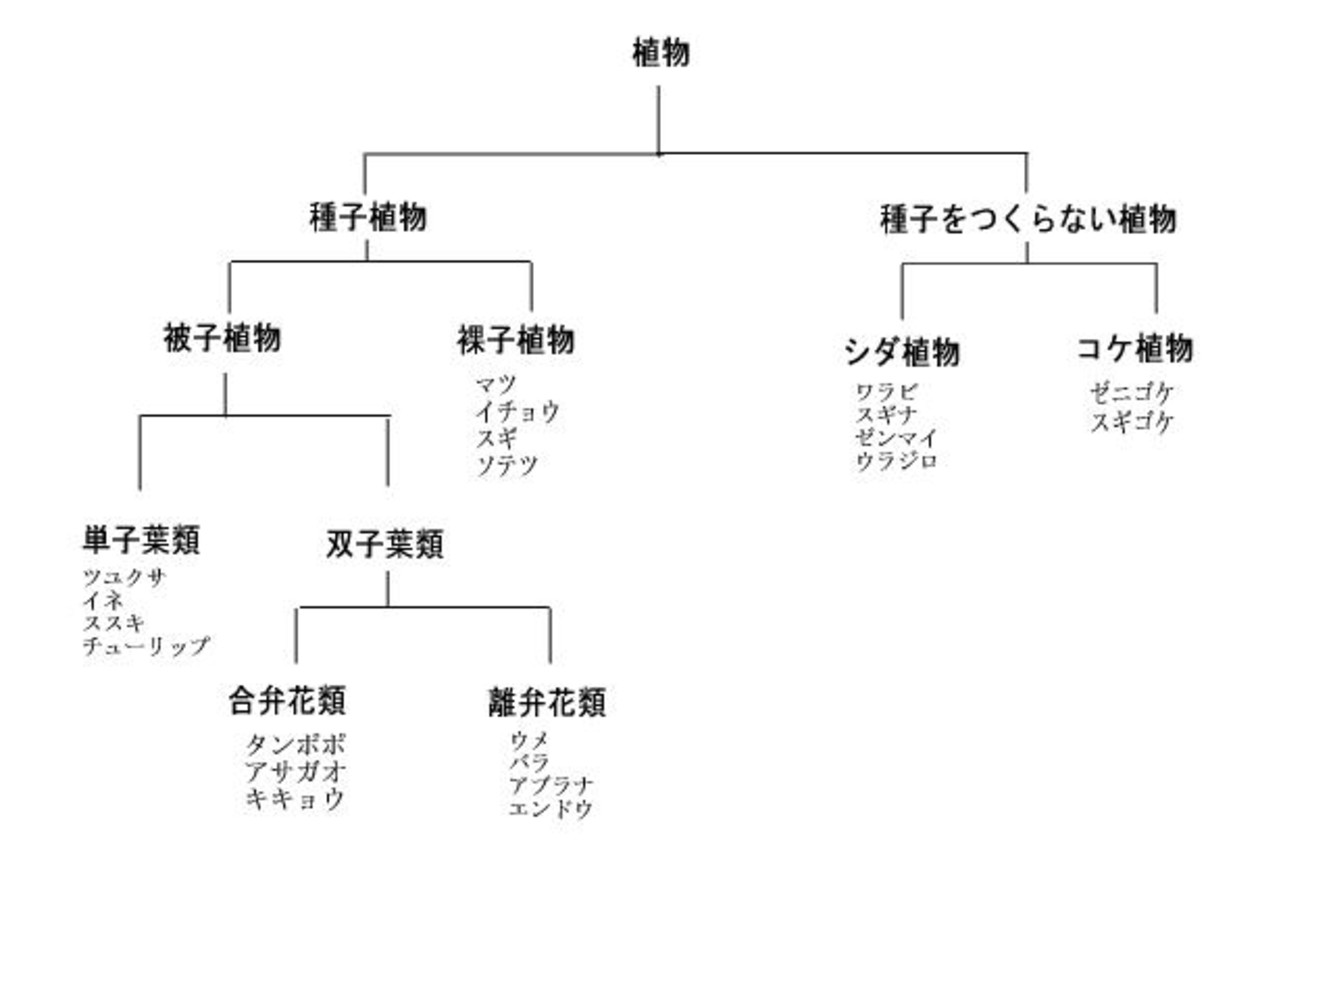
\includegraphics[height=10cm]{science_figure/bunrui.pdf}
	}
\end{itembox}

\begin{itembox}[l]{子葉、維管束、葉脈、根の分類}
	{\renewcommand\arraystretch{\page{1}{2}}
		\centering
		\begin{tabular}{|l||p{6cm}|p{6cm}|}
			\hline
			         & \answer{0}{単子葉類}                 & \answer{0}{双子葉類}       \\
			\hline
			\hline
			子葉     & \answer{0}{1枚}                      & \answer{0}{2枚}            \\
			\hline
			維管束   & \answer{0}{バラバラに散らばっている} & \answer{0}{輪に並んでいる} \\
			\hline
			葉脈     & \answer{0}{平行脈}                   & \answer{0}{網状脈}         \\
			\hline
			根の分類 & \answer{0}{ひげ根}                   & \answer{0}{主根と側根}     \\
			\hline
		\end{tabular}
	}
\end{itembox}

\begin{itembox}[l]{維管束は何からなるか、内側・外側}
	\answer{10}{維管束は道管と師管、茎において道管が内側、葉において裏側が道管}
\end{itembox}


\begin{itembox}[l]{根毛がある理由}
	\answer{10}{表面積を大きくして、効率よく水分や栄養を根から吸収するため}
\end{itembox}

\begin{itembox}[l]{気孔の役割、周辺にある細胞、どこからが一番蒸散するか}
	\answer{10}{蒸散を行ったり、酸素や二酸化炭素の出入りに使われる。孔辺細胞。葉の裏側}
\end{itembox}



\section{2年の生物}
\begin{itembox}[l]{有名な臓器とその役割(7)}
	\question{
		\Large{
			\begin{itemize}
				\item \item \item \item \item \item \item
			\end{itemize}
		}
	}{
		\begin{itemize}
			\item 心臓:血液を全身に送り出す
			\item 肺:空気中の酸素を取り込み、血液中の二酸化炭素を排出する
			\item 胃:消化
			\item 小腸:栄養を吸収する
			\item 大腸:水分を吸収する
			\item 肝臓:胆汁をつくる、血液中のアンモニアを尿素に変える。
			\item 胆のう:胆汁をたくわえる
			\item 腎臓:血液中の老廃物(尿素)をこしとる。ぼうこうに溜められ尿として排出
		\end{itemize}
	}
\end{itembox}


\begin{itembox}[l]{小腸の壁の突起物の名前とその役割}
	\answer{10}{柔毛、表面積を大きくして効率よく栄養を吸収するため}
\end{itembox}

\begin{itembox}[l]{消化後何になるか、どこに吸収されるか}
	\answer{10}{
		炭水化物$\rightarrow$麦芽糖$\rightarrow$ブドウ糖$\rightarrow$毛細血管\\
		タンパク質$\rightarrow$アミノ酸$\rightarrow$ 毛細血管\\
		脂肪$\rightarrow$脂肪酸とモノグリセリド$\rightarrow$ 脂肪に戻ってリンパ管
	}
\end{itembox}

\begin{itembox}[l]{消化酵素と分解後の物質}
	\answer{20}{
		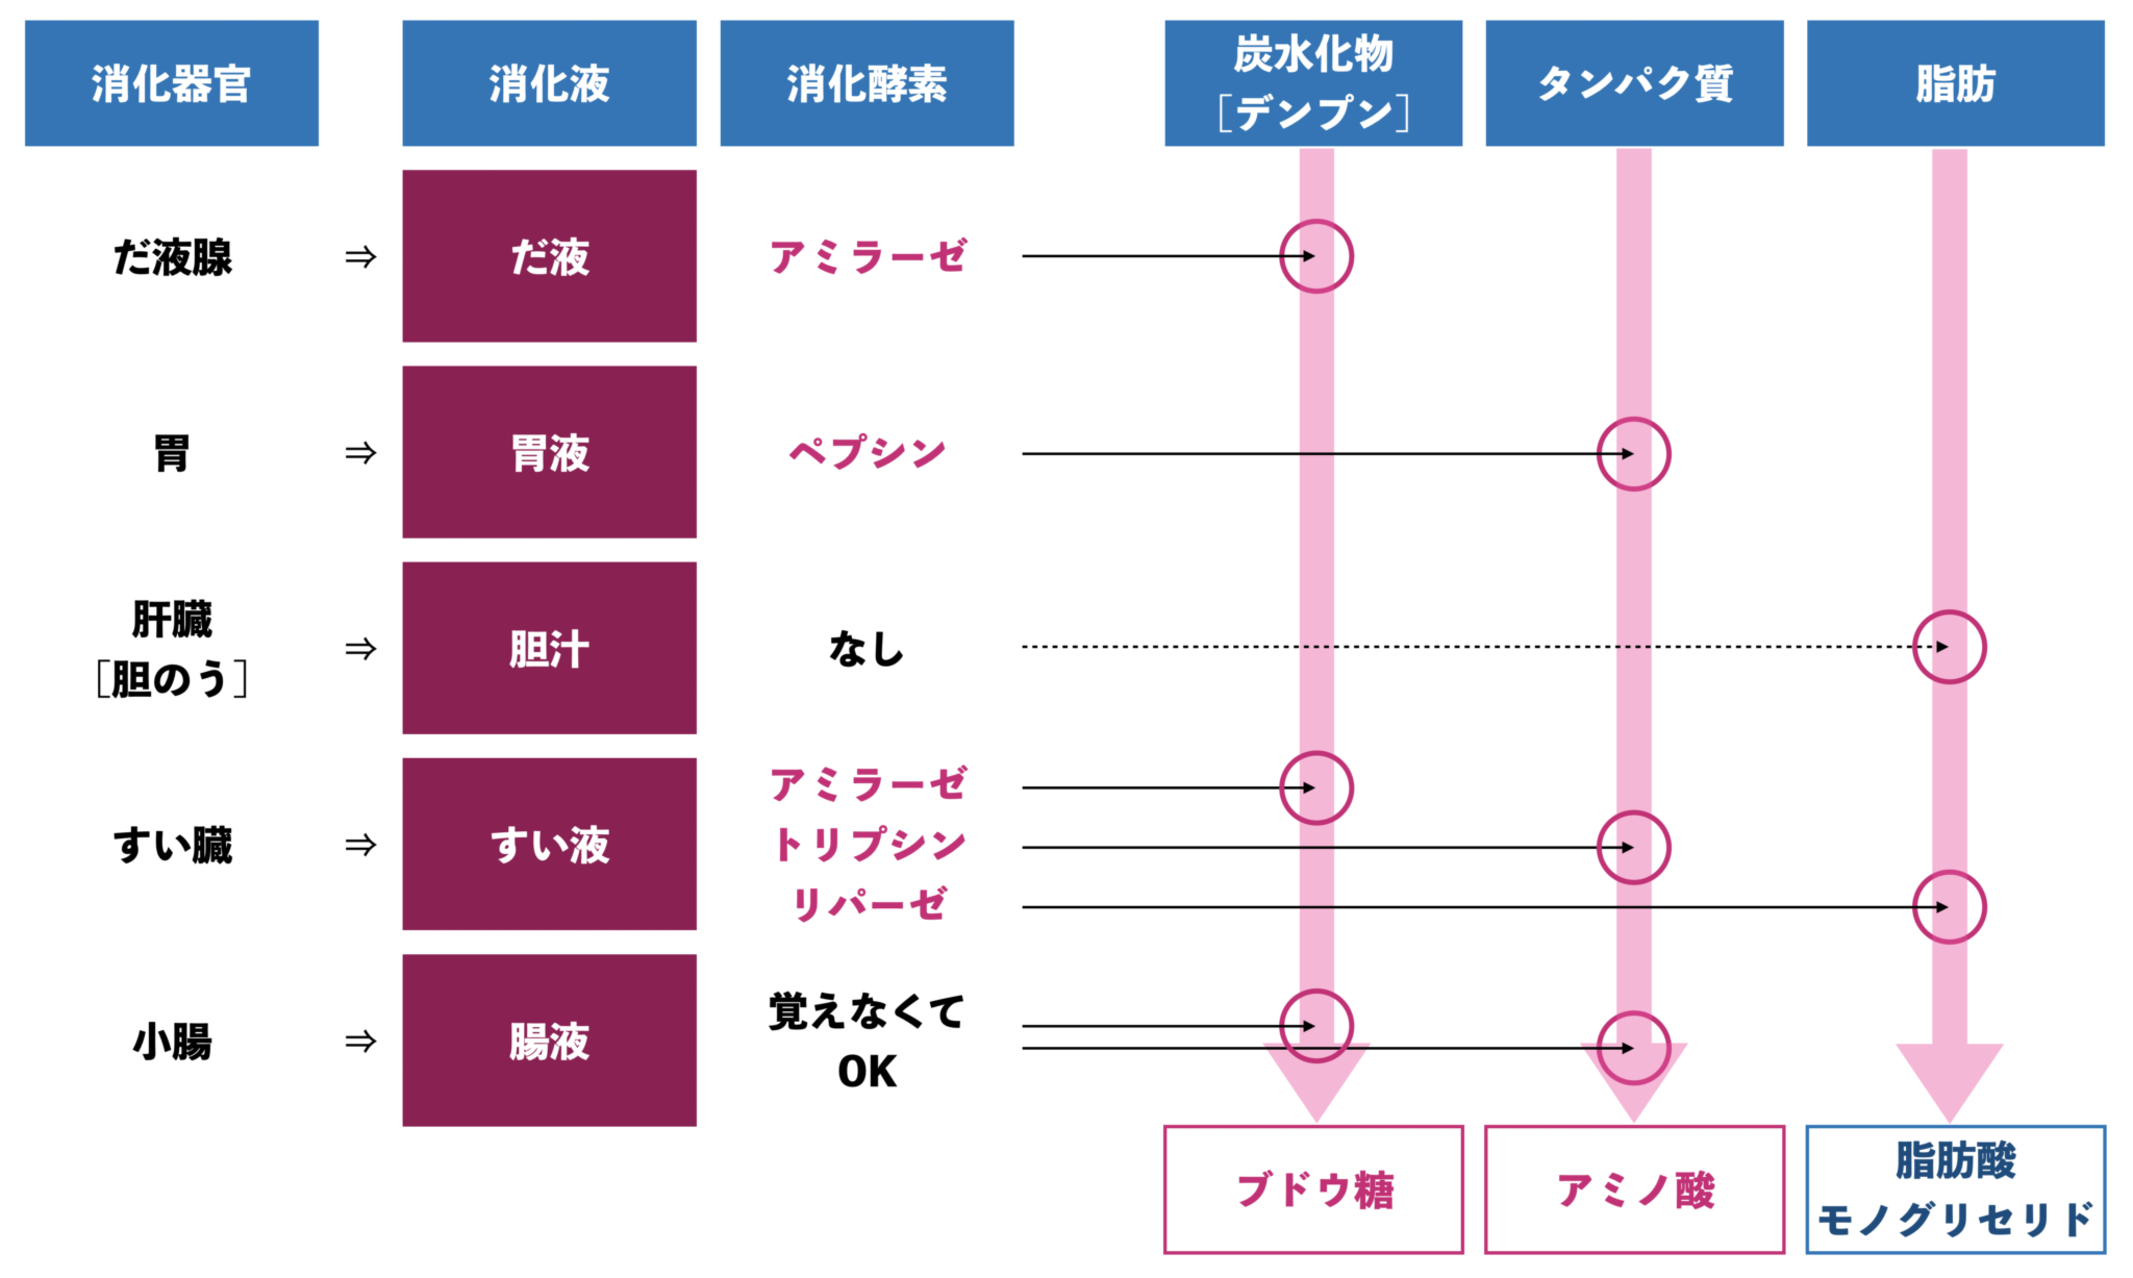
\includegraphics[width=10cm]{science_figure/syoka.pdf}
	}
\end{itembox}

\begin{itembox}[l]{肺にある小さな部屋の名前とその役割}
	\answer{10}{肺胞、表面積を大きくして効率よく酸素を吸収するため}
\end{itembox}

\begin{itembox}[l]{動脈と動脈血の違い、動脈血が流れる静脈はどこ}
	\answer{10}{
		動脈$\rightarrow$心臓から出ていく血管、\\
		動脈血$\rightarrow$酸素を多く含んだ血液、\\
		肺静脈は肺で酸素を吸収するため酸素を多く含んでいる\\
	}
\end{itembox}

\begin{itembox}[l]{血管の特徴}
	\answer{8}{
		動脈$\rightarrow$心臓から出ていく勢いに耐えるため壁が厚い、\\
		静脈$\rightarrow$逆流を防ぐために弁がある。
	}
\end{itembox}

\begin{itembox}[l]{反射と反射以外の反応、中枢神経と末しょう神経、情報が伝わる経路}
	\answer{15}{
		反射は無意識で脳で判断されない\\
		中枢神経は脊髄と脳、末しょう神経は感覚神経と運動神経\\
		反射以外:感覚器官$\rightarrow$感覚神経$\rightarrow$脊髄$\rightarrow$脳$\rightarrow$脊髄$\rightarrow$運動神経$\rightarrow$運動器官\\
		反射:感覚器官$\rightarrow$感覚神経$\rightarrow$脊髄$\rightarrow$運動神経$\rightarrow$運動器官

	}
\end{itembox}


\section{3年の生物}
\begin{itembox}[l]{体細胞分裂と減数分裂の違い、起こるタイミング}
	\answer{10}{
		体細胞分裂$\rightarrow$成長するために行われ細胞の数が増える、染色体の数は変わらない\\
		減数分裂$\rightarrow$生殖細胞を作るために行われる、染色体の数が半分になる
	}
\end{itembox}

\begin{itembox}[l]{根の成長、場所}
	\answer{10}{細胞分裂によって細胞の数が増え、一つ一つの細胞が大きくなることで成長する。細胞分裂は根の先端付近でよく起こるが、先端は根冠であり、少し硬い。}
\end{itembox}

\begin{itembox}[l]{胚と発生の違い}
	\answer{10}{
		胚$\rightarrow$受精後に細胞分裂が行われ自分で餌を食べれるようになるまでの状態\\
		発生$\rightarrow$胚が細胞分裂を行なって成長していく過程
	}
\end{itembox}

\begin{itembox}[l]{顕性形質と潜性形質、対立形質の違い}
	\answer{10}{
		対立形質$\rightarrow$同時には現れない生物の形質\\
		顕性形質$\rightarrow$現れやすい形質\\
		潜性形質$\rightarrow$現れにくい形質
	}
\end{itembox}

\begin{itembox}[l]{純系同士の交配、子の交配}
	\begin{multicols}{2}
		\begin{minipage}{0.5\textwidth}
			純系同士の交配\\
			{\renewcommand\arraystretch{2}
			\begin{tabular}[h]{p{1cm}|p{1.5cm}|p{1.5cm}|}
				 &  & \\
				\hline
				 &  & \\
				\hline
				 &  & \\
				\hline
			\end{tabular}
			}
		\end{minipage}
		\begin{minipage}{0.5\textwidth}
			子の交配\\
			{\renewcommand\arraystretch{2}
			\begin{tabular}[h]{p{1cm}|p{1.5cm}|p{1.5cm}|}
				 &  & \\
				\hline
				 &  & \\
				\hline
				 &  & \\
				\hline
			\end{tabular}
			}
		\end{minipage}
	\end{multicols}
\end{itembox}


\begin{itembox}[l]{生態系}
	\answer{20}{
		\begin{description}
			\item[生産者] 植物、光合成
			\item[消費者] 動物、他の生物を食べることで生きる
			\item[分解者] 有機物を無機物に分解する生物。
		\end{description}
		どの生物も呼吸を行っている。
	}
\end{itembox}


\newpage

\section{1年の化学}

\begin{itembox}[l]{無機物と有機物}
	\answer{10}{
		無機物$\rightarrow$有機物以外、金属\\
		有機物$\rightarrow$水素と炭素を含む物質、燃やすと水と二酸化炭素が発生
	}
\end{itembox}

\begin{itembox}[l]{気体の収集方法とそれぞれを使う基準}
	\answer{20}{
		水上置換法$\rightarrow$水に溶けにくい物質\\
		上方置換法$\rightarrow$水に溶けやすく、空気より軽い物質\\
		下方置換法$\rightarrow$水に溶けやすく、空気より重い物質

	}
\end{itembox}


\begin{itembox}[l]{気体の発生方法(何に何を入れるか)、回収方法}

	{\renewcommand\arraystretch{\page{1}{2}}
		\centering
		\begin{tabular}{|c|p{3cm}|p{3cm}|p{2.5cm}|p{4.5cm}|}
			\hline
			           & 液体                                         & 固体                                           & 回収方法                               & 確認方法                                                 \\
			\hline
			\hline
			水素       & \answer{0}{塩酸}                             & \answer{0}{亜鉛などの金属}                     & \answer{0}{水上置換法}                 & \answer{0}{火の付けたマッチを近づけて音を立てて燃えるか} \\
			\hline
			酸素       & \answer{0}{うすい過酸化水素水かオキシドール} & \answer{0}{二酸化マンガン}                     & \answer{0}{水上置換法}                 & \answer{0}{火のついた線香が激しく燃えるか}               \\
			\hline
			二酸化炭素 & \answer{0}{塩酸}                             & \answer{0}{石灰石}                             & \answer{0}{水上置換法または下方置換法} & \answer{0}{石灰水が白くにごるか}                         \\
			\hline
			アンモニア & \answer{0}{}                                 & \answer{0}{塩化アンモニウムと水酸化カルシウム} & \answer{0}{上方置換法}                 & \answer{0}{刺激臭}                                       \\
			\hline
		\end{tabular}
	}
\end{itembox}





\begin{itembox}[l]{溶液・溶質・溶媒、食塩水においてどれがどれか}
	\answer{10}{
		食塩水が溶液、食塩が溶質、水が溶媒
	}
\end{itembox}

\begin{itembox}[l]{溶解度とはなにか}
	\answer{10}{
		100gの水に溶ける限界の量、水の量が違えば比の計算
	}
\end{itembox}

\begin{itembox}[l]{公式(単位も)}
	\begin{Large}
		\begin{itemize}
			\item 密度 \answer{0}{$\frac{質量(g)}{体積(cm^3)}$、$g/cm^3$}
			\item 質量パーセント濃度 \answer{0}{$\frac{溶質}{溶液}$}
		\end{itemize}
	\end{Large}
\end{itembox}

\begin{itembox}[l]{物質の取り出し方}
	\begin{Large}
		\begin{itemize}
			\item 再結晶 \answer{0}{
				      \normalsize 温めながら水に溶かして、冷やして結晶にして取り出す、溶解度の違いを利用}
			\item 蒸留 \answer{0}{\normalsize 蒸発させて、冷やして液体として取り出す、沸点の違いを利用}
			\item ろ過 \answer{0}{\normalsize 混ざっていないいらないものを取り出す、ろしとろうと}
		\end{itemize}
	\end{Large}
\end{itembox}

\newpage

\section{2年の化学}
\begin{itembox}[l]{状態変化と化学変化}
	\answer{10}{
		状態変化$\rightarrow$固体・液体・気体に変化すること、物質名は変わらない\\
		化学変化$\rightarrow$全く別の物質になる、化合や分解
	}
\end{itembox}



\begin{itembox}[l]{分子をつくる物質、つくらない物質}
	\answer{10}{
		分子を作る物質$\rightarrow$固体・液体・気体に変化すること、物質名は変わらない\\
		分子を作らない物質$\rightarrow$全く別の物質になる、化合や分解
	}
\end{itembox}

\begin{itembox}[l]{炭酸水素ナトリウムの熱分解の実験で気をつけるポイントとその理由 2つ}
	\begin{Large}
		\begin{itemize}
			\item \answer{0}{\normalsize 試験管の口を下げる、発生した液体が加熱部に流れて試験管が割れるのを防ぐ}
			\item \answer{0}{\normalsize 加熱を止める前にガラス管を水から抜く、逆流して試験管が割れるのを防ぐ}
		\end{itemize}
	\end{Large}
\end{itembox}

\begin{itembox}[l]{硫黄と鉄の反応で反応が続く理由}
	\answer{10}{反応によって熱が発生し、その熱で次の反応が起こるから}
\end{itembox}

\begin{itembox}[l]{硫黄と鉄の混合物の加熱前と加熱後の物質の違い(結果も含む)、4つ}

	{\renewcommand\arraystretch{\page{1}{2}}
		\centering
		\begin{tabular}{|p{5cm}||p{4cm}|p{4cm}|}
			\hline
			\diagbox{確認方法}{物質名}   & 加熱前                               & 加熱後(\page{硫化鉄}{       } ) \\
			\hline
			\hline
			\answer{0}{塩酸の中に入れる} & \answer{0}{水素が発生、匂いはしない} & \answer{0}{硫化水素が発生、腐卵臭}     \\
			\hline
			\answer{0}{磁石を近づける}   & \answer{0}{ひっつく}                 & \answer{0}{ひっつかない}               \\
			\hline
			\answer{0}{電流を流す}       & \answer{0}{流れる}                   & \answer{0}{流れない}                   \\
			\hline
			\answer{0}{色}               & \answer{0}{銀白色と黄色の混合物}     & \answer{0}{黒色}                       \\
			\hline
		\end{tabular}
	}
\end{itembox}

\begin{itembox}[l]{気体の確認方法}
	\begin{Large}
		\begin{itemize}
			\item 硫化水素 \answer{0}{\normalsize 手で仰ぐように嗅ぐ、腐卵臭}
		\end{itemize}
	\end{Large}
\end{itembox}

\begin{itembox}[l]{水の電気分解ポイント}
	\answer{10}{純粋な水には電流が流れないので、水酸化ナトリウムを溶かす}
\end{itembox}

\begin{itembox}[l]{酸化銅と炭素を用いた還元の実験で気をつけるポイントとその理由}
	\answer{10}{反応終了後にゴム管をピンチコックでつまむ、酸素と物質が触れないようにするため}
\end{itembox}

\begin{itembox}[l]{質量保存の法則、成り立つとき・成り立たないとき}
	\answer{10}{密閉されずに行われ、気体が発生すると成立していないように見える}
\end{itembox}

\section{3年の化学}
\begin{itembox}[l]{電解質とはどのような物質か}
	\answer{10}{水に溶かした時に電離する物質、水溶液に電流が流れる}
\end{itembox}

\begin{itembox}[l]{電離とは}
	\answer{10}{陽イオンと陰イオンに分かれること}
\end{itembox}

\begin{itembox}[l]{イオン化傾向とは}
	\answer{10}{イオンへのなりやすさ}
\end{itembox}
\begin{itembox}[l]{電池の仕組み}
	\answer{10}{
		亜鉛板と銅板を塩酸の中に入れた場合
		\begin{enumerate}
			\item 亜鉛と銅では亜鉛の方がイオンになりやすいので、亜鉛原子が亜鉛イオンとなり水中に溶け出す
			\item 亜鉛イオンになる際に出てきた電子が銅板に流れ込む
			\item 銅イオンが電子を受け取り銅原子になり付着する
		\end{enumerate}
	}
\end{itembox}

\begin{itembox}[l]{酸・アルカリの定義}
	\answer{10}{
		酸$\rightarrow$水に溶かした時に水素イオンを生じる\\
		アルカリ$\rightarrow$水に溶かした時に水酸化物イオンを生じる
	}
\end{itembox}

\begin{itembox}[l]{酸・アルカリの確認方法 4つ}

	{\renewcommand\arraystretch{\page{1}{2}}
		\centering
		\begin{tabular}{|p{4cm}||p{3cm}|p{3cm}|p{3cm}|}
			\hline
			試薬名                           & 酸                       & 中性                 & アルカリ性               \\
			\hline
			\hline
			\answer{0}{BTB溶液}              & \answer{0}{黄色}         & \answer{0}{緑色}     & \answer{0}{青色}         \\
			\hline
			\answer{0}{リトマス試験紙}       & \answer{0}{青色が赤色に} & \answer{0}{変化なし} & \answer{0}{赤色が青色に} \\
			\hline
			\answer{0}{フェノールフタレイン} & \answer{0}{変化なし}     & \answer{0}{変化なし} & \answer{0}{赤色}         \\
			\hline
			\answer{0}{金属を入れる}         & \answer{0}{水素が発生}   & \answer{0}{変化なし} & \answer{0}{変化なし}     \\
			\hline
		\end{tabular}
	}
\end{itembox}

\begin{itembox}[l]{pHとは、値が表す意味}
	\answer{10}{
		酸やアルカリの強さを示す、中性の時7、小さければ強い酸性、大きければ強いアルカリ性
	}
\end{itembox}

\begin{itembox}[l]{中和とはなにか、沈殿が生じるやつ}
	\answer{10}{
		酸の水素イオンとアルカリの水酸化物イオンから水ができること、水以外にできるものを塩、硫酸と水酸化バリウムを混合すると白色の沈殿ができる。
	}
\end{itembox}

\newpage

\section{1年の物理}
\begin{itembox}[l]{焦点距離とは}
	\answer{10}{
		レンズの中心から焦点までの距離
	}
\end{itembox}

\begin{itembox}[l]{実像ができる場合、図を書く}
	\answer{20}{
		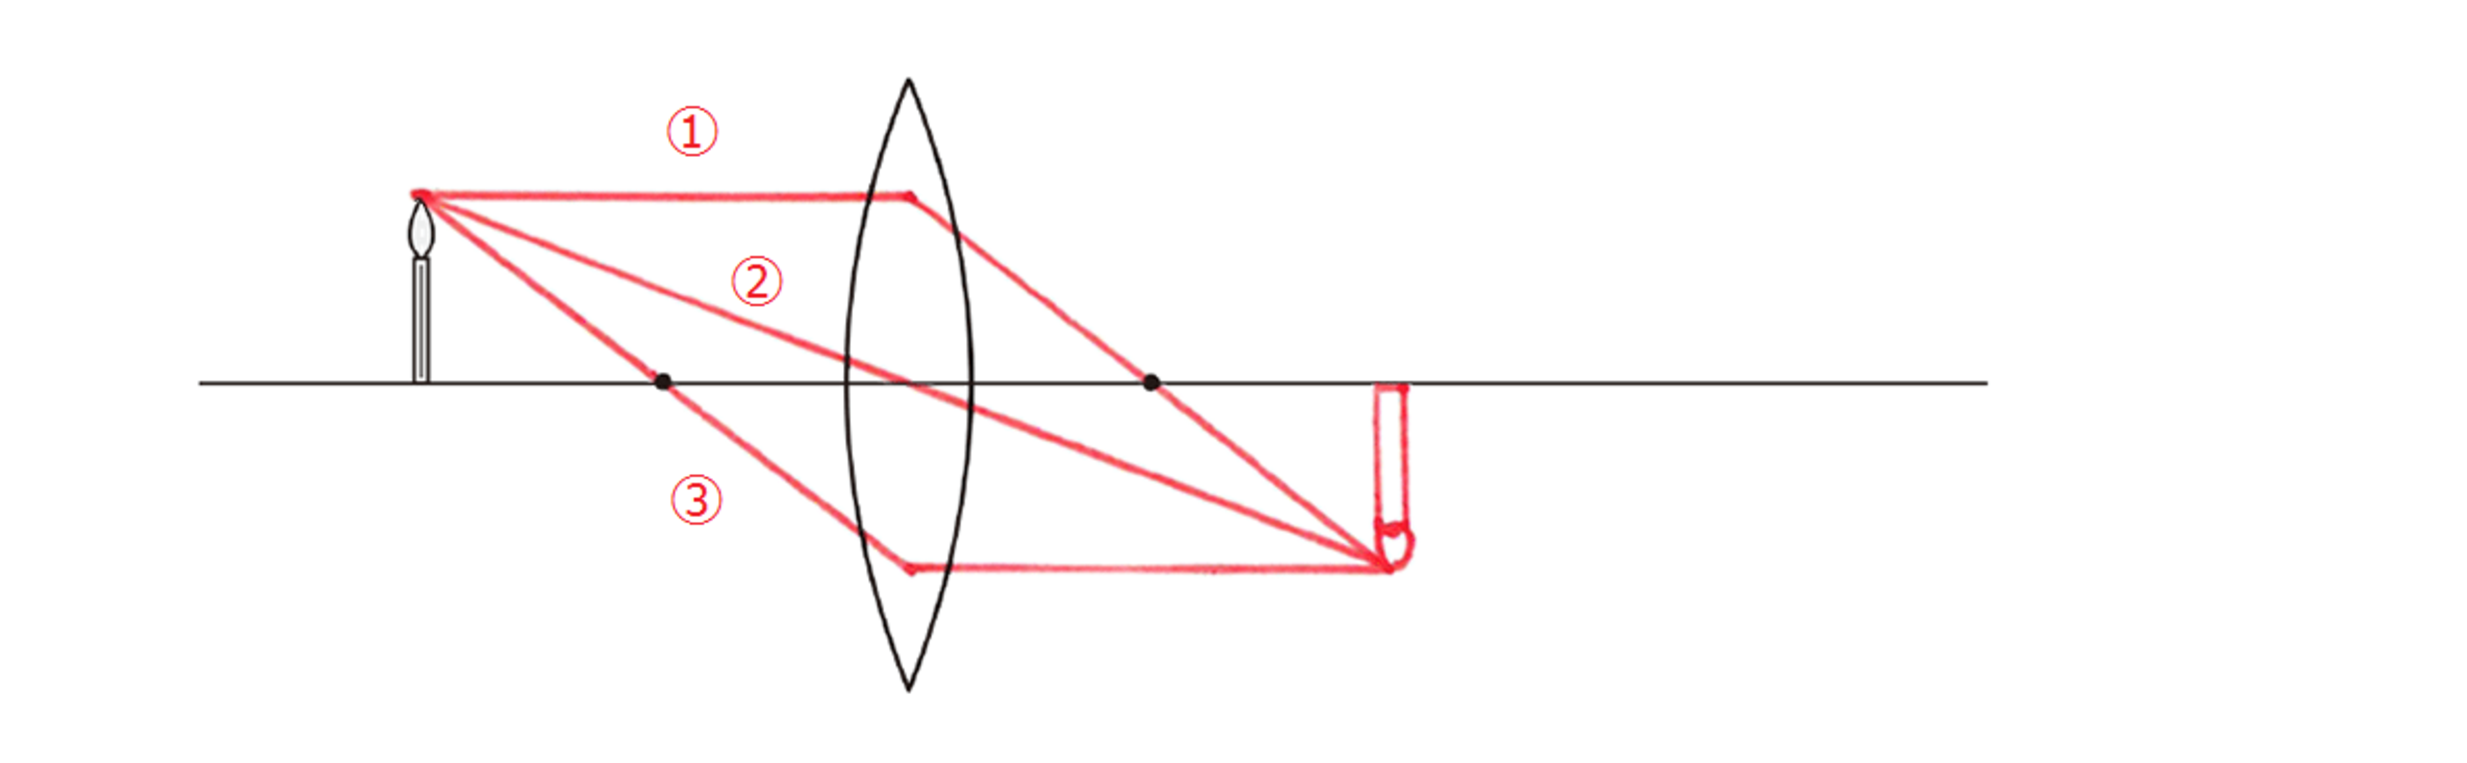
\includegraphics[height=5cm]{science_figure/zituzo.pdf}
	}
\end{itembox}

\begin{itembox}[l]{虚像ができる場合、図を書く}
	\answer{20}{
		焦点より内側にある時にできる
		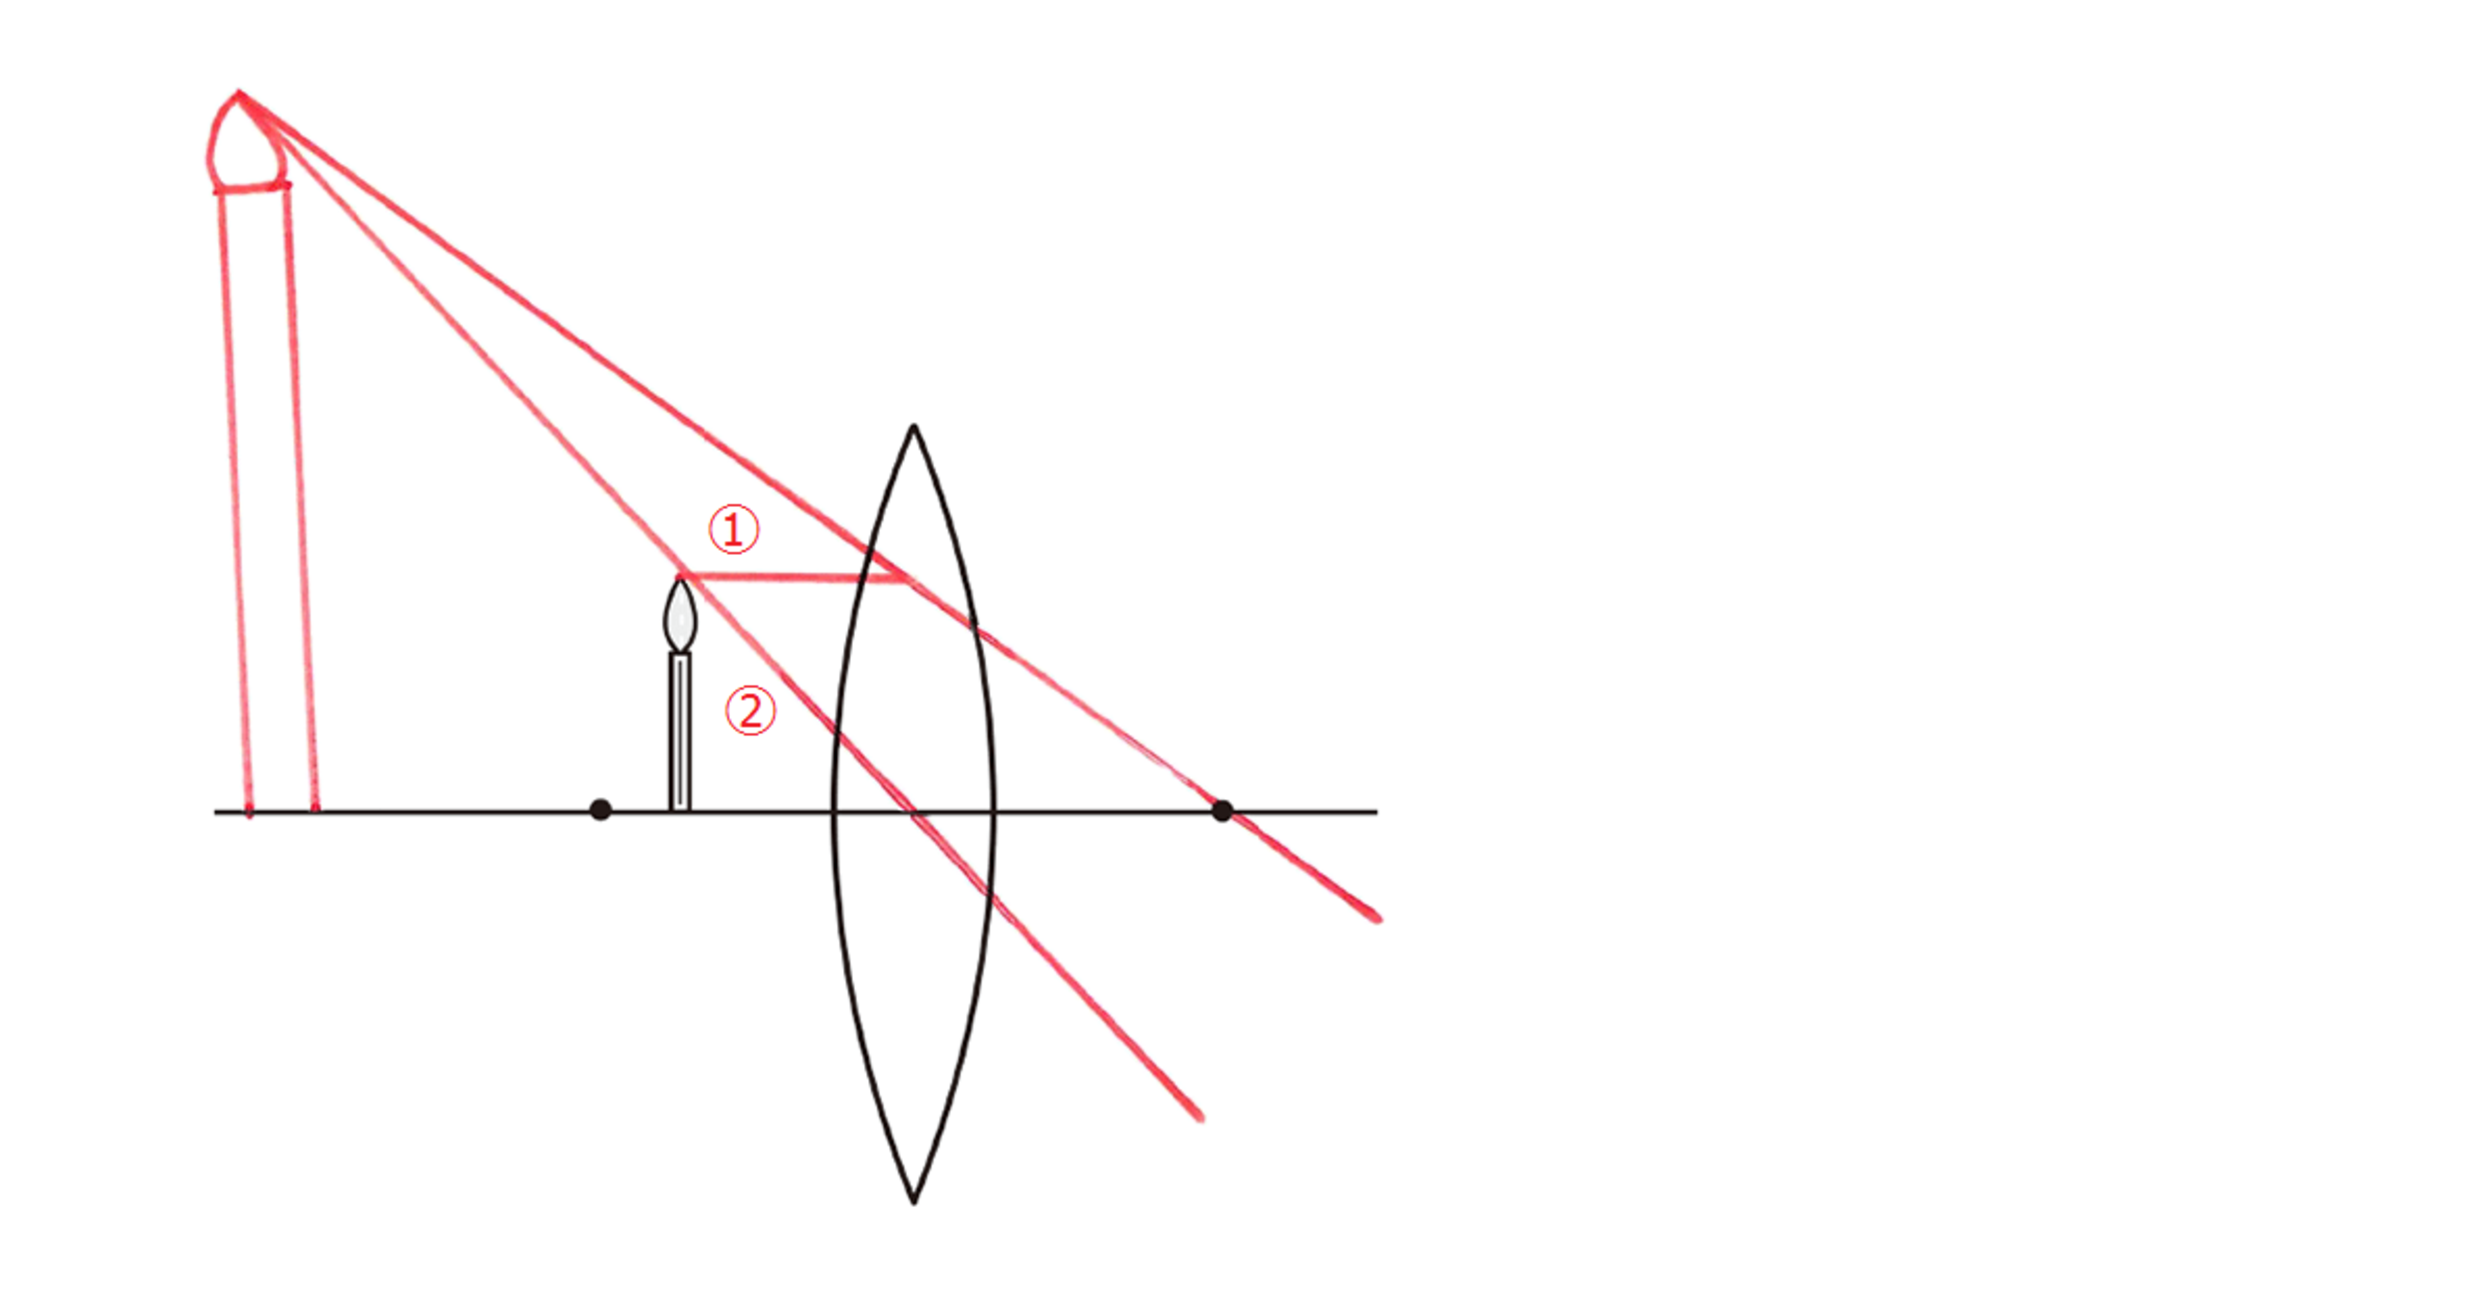
\includegraphics[height=5cm]{science_figure/kyozo.pdf}
	}
\end{itembox}

\begin{itembox}[l]{像の大きさについて}
	\answer{30}{
		実像$\rightarrow$左右上下反転、焦点距離の2倍なら物体と同じ大きさ、2倍より遠ければ小さい、近ければ大きい\\
		虚像$\rightarrow$同じ向き、大きい
	}
\end{itembox}

\begin{itembox}[l]{花火の音が遅れる理由}
	\answer{10}{光速に比べて音速が遅いから}
\end{itembox}

\begin{itembox}[l]{音の高さと大きさそれぞれの原因}
	\answer{10}{
		音の高さ$\rightarrow$振動数、波の数\\
		音の大きさ$\rightarrow$振幅、波の幅
	}
\end{itembox}

\begin{itembox}[l]{テーブルの上にある物体を横に引っ張るときに働く力(物体に働く力は全てかくこと)。机はなめらかではない}
	\vspace{3cm}
\end{itembox}

\newpage

\section{2年の物理}
\begin{itembox}[l]{電流の正体と流れる方向、正体の流れる方向}
	\begin{Large}
		\begin{itemize}
			\item 電流 \answer{0}{\normalsize +極から-極}
			\item 電流の正体 \answer{0}{\normalsize 電子、-極から+極}
		\end{itemize}
	\end{Large}
\end{itembox}

\begin{itembox}[l]{電流計と電圧計の使い方}
	\answer{10}{
		電流計$\rightarrow$測定したいものに対して直列\\
		電圧計$\rightarrow$測定したいものに対して並列
	}
\end{itembox}

\begin{itembox}[l]{直列と並列の違い、それぞれの合成抵抗}
	{\renewcommand\arraystretch{\page{1}{2}}
		\centering
		\begin{tabular}{|c||p{4cm}|p{4cm}|p{4cm}|}
			\hline
			     & 電圧             & 電流             & 合成抵抗             \\
			\hline
			直列 &                  & \answer{0}{同じ} & \answer{0}{和}       \\
			\hline
			並列 & \answer{0}{同じ} &                  & \answer{0}{逆数の和} \\
			\hline
		\end{tabular}
	}
\end{itembox}

\begin{itembox}[l]{電磁誘導とは、いつ起きる}
	\answer{20}{コイル内の磁界が変化するとおきる、誘導電流が流れる}
\end{itembox}

\begin{itembox}[l]{公式(単位も)}
	\begin{Large}
		\begin{itemize}
			\item オームの法則 \answer{0}{$V=RI$}
			\item 電力 \answer{0}{$W=VI、 W$}
			\item 熱量(電力量) \answer{0}{$W\times s、J$}
		\end{itemize}
	\end{Large}
\end{itembox}

\newpage

\section{3年の物理}
\begin{itembox}[l]{水圧と浮力、それぞれの原因と何に比例するか}
	\answer{10}{
		水圧$\rightarrow$物体が沈んでいる深さに依存する\\
		浮力$\rightarrow$物体の沈んでいる体積に依存する、上面と下面にかかる水圧の差によって生まれる
	}
\end{itembox}

\begin{itembox}[l]{慣性とは}
	\answer{10}{
		静止している物体が静止し続け、動いている物体が等速直線運動を続ける性質
	}
\end{itembox}

\begin{itembox}[l]{力の釣り合いと作用反作用の法則}
	\answer{10}{
		つりあい$\rightarrow$一つの物体に対してかかる\\
		作用・反作用$\rightarrow$二つの物体に対して互いにかかる
	}
\end{itembox}

\begin{itembox}[l]{斜面の物体(5N)、斜面の物体に働く力とその分解}
	\begin{center}
		\begin{tikzpicture}[scale=1]
			\coordinate (A) at (0,0);
			\coordinate (B) at ({3*sqrt(3)},0);
			\coordinate (C) at ({3*sqrt(3)},3);
			\draw (0,0)--({3*sqrt(3)},0)--({3*sqrt(3)},3)--cycle;
			\draw[rotate around={30:({sqrt(3)},1)}] ({sqrt(3)},1) rectangle ({2*sqrt(3)},2);
			\draw pic[draw=black, angle eccentricity=1.3, angle radius=1cm]{angle=B--A--C};
			\node[above right] at (1,0.2) {30\textdegree};
		\end{tikzpicture}
	\end{center}

\end{itembox}

\begin{itembox}[l]{動滑車と定滑車}
	\answer{10}{
		定滑車$\rightarrow$力のむきを変える\\
		動滑車$\rightarrow$力の大きさは半分になるが、引く長さが倍になる
	}
\end{itembox}

\begin{itembox}[l]{仕事の原理とは}
	\answer{10}{
		仕事の前後の位置が同じであれば、どのように計算しても仕事の量は変わらない
	}
\end{itembox}

\begin{itembox}[l]{公式(単位も)}
	\begin{Large}
		\begin{itemize}
			\item 仕事 \answer{0}{$N\times m、J$}
			\item 仕事率 \answer{0}{$J/s、 W$}
		\end{itemize}
	\end{Large}
\end{itembox}

\begin{itembox}[l]{力学的エネルギーとは、特徴}
	\answer{10}{
		運動エネルギーと位置エネルギーの和、常に一定
	}
\end{itembox}

\newpage

\section{1年の地学}
\begin{itembox}[l]{海辺から遠くなる程、石の大きさはどうなるか}
	\answer{10}{小さくなる}
\end{itembox}

\begin{itembox}[l]{石灰岩とチャートの見分け方}
	\answer{10}{石灰岩は塩酸をかけると二酸化炭素が発生}
\end{itembox}

\begin{itembox}[l]{示準化石と示相化石の説明}
	\answer{10}{
		示相化石$\rightarrow$当時の周りの様子がわかる、現代にも生きているが特定の環境のみ\\
		示準化石$\rightarrow$どの年代かがわかる、現代にないのがポイント
	}
\end{itembox}

\begin{itembox}[l]{地震の波の種類(2)}
	\answer{10}{
		初期微動(P波)、主要動(S波)
	}
\end{itembox}

\begin{itembox}[l]{火成岩2種類、それらの違い、組織名}
	\answer{10}{
		火山岩$\rightarrow$地表付近で急激に冷えて生成\\
		深成岩$\rightarrow$近深くでゆっくりと冷えて生成
	}
\end{itembox}

\begin{itembox}[l]{溶岩によってできる岩石の分類}
	\answer{30}{
		しんかんせんはかりあげ\\
		深成岩、かこう岩、閃緑岩、はんれい岩、火山岩、流紋岩、安山岩、玄武岩
	}
\end{itembox}


\section{2年の地学}
\begin{itembox}[l]{露点とはなにか}
	\answer{10}{
		空気中に含まれている水分が飽和水蒸気量と同じになる温度
	}
\end{itembox}

\begin{itembox}[l]{高気圧と低気圧、上昇気流・下降気流、風のむき}
	\answer{10}{
		高気圧$\rightarrow$周りに比べて気圧が高い、下降気流\\
		低気圧$\rightarrow$周りに比べて気圧が低い、上昇気流\\
		右ねじの法則で吹き出したり吹き込む風の向きがわかる\\
		高気圧から低気圧に向かって風は吹く
	}
\end{itembox}

\begin{itembox}[l]{雲のでき方}
	\answer{10}{
		\begin{enumerate}
			\item 空気が持ち上げられる
			\item 空気が冷やされて、露点に達する
			\item 空気中の水蒸気が水になる
		\end{enumerate}
	}
\end{itembox}

\begin{itembox}[l]{前線(4)}
	\answer{10}{
		\begin{description}
			\item[寒冷前線] 寒気の方が強い、温度が下がり、風向が北寄り、積乱雲(短い時間に狭い範囲で強い雨)
			\item[温暖前線] 暖気の方が強い、温度が上がり、風向が南寄り、乱層雲(長い時間に広い範囲で弱い雨)
			\item[閉塞前線] 寒冷前線が温暖前線に追いつく
			\item[停滞前線] 梅雨前線・秋雨前線などの長い期間停滞して雨を降らせる、ほとんど動かない
		\end{description}
	}
\end{itembox}

\begin{itembox}[l]{温帯低気圧}
	\answer{30}{
		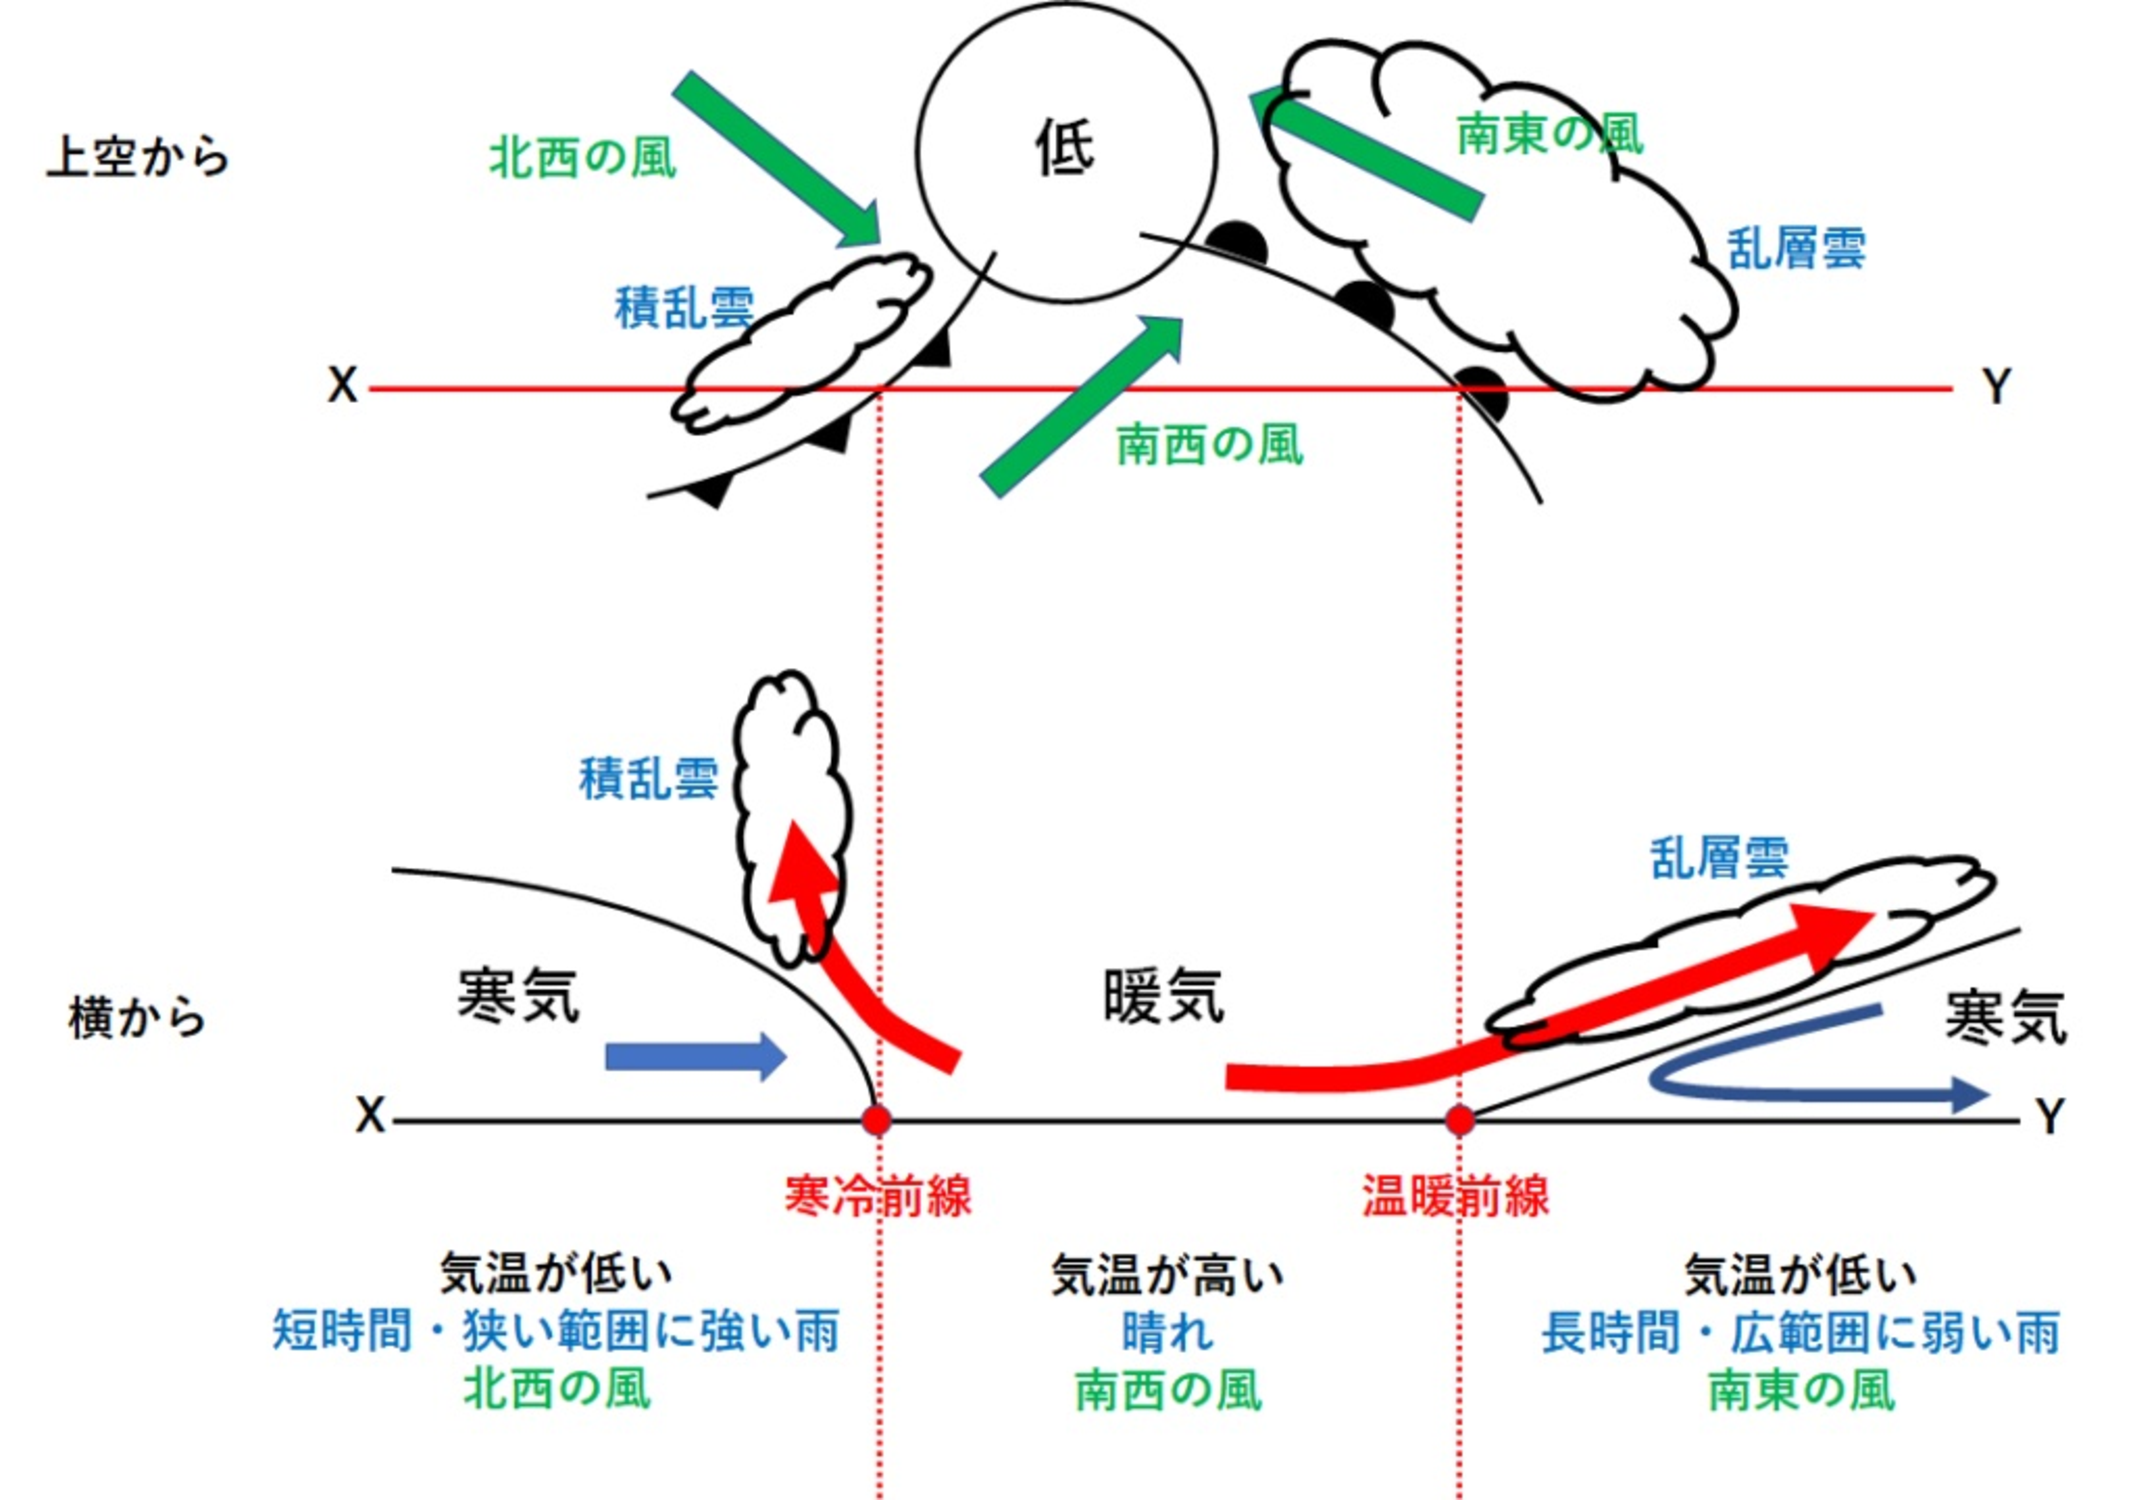
\includegraphics[height=10cm]{science_figure/typhoo.pdf}\\
		寒冷前線はいずれ温帯低気圧に追いついて閉塞前線になる
	}
\end{itembox}

\begin{itembox}[l]{公式(単位も)}
	\begin{Large}
		\begin{itemize}
			\item 圧力 \answer{0}{$\frac{N}{m^2}、Pa$}
			\item 湿度 \answer{0}{$\frac{含んでいる量}{含める量}\times100$}
		\end{itemize}
	\end{Large}
\end{itembox}


\section{3年の地学}
\begin{itembox}[l]{南中と南中高度}
	\answer{10}{南中とは太陽が真南にきて1日で最も高い位置に来ること\\
		南中高度は太陽が南中した時の南を向いて太陽までの角度}
\end{itembox}

\begin{itembox}[l]{秋分、夏至、春分、冬至の説明}
	\answer{20}{
		\begin{itemize}
			\item 春分・秋分 昼と夜の長さが同じ、真東から登って真西に沈む
			\item 夏至 昼が長い、北よりから登って沈む、南中高度が最大
			\item 冬至 夜が長い、南よりから登って沈む、南中高度が最小
		\end{itemize}
	}
\end{itembox}

\begin{itembox}[l]{恒星、衛星、惑星}
	\answer{15}{
		\begin{itemize}
			\item 恒星 自ら光を放つもの
			\item 惑星 恒星の周りを公転するもの
			\item 衛星 惑星の周りを公転するもの
		\end{itemize}
	}
\end{itembox}

\begin{itembox}[l]{太陽系と太陽系外縁天体}
	\answer{15}{太陽系は水金地火木土天海\\
		冥王星は太陽系外縁天体}
\end{itembox}

\begin{itembox}[l]{年周運動と日周運動の違いと原因、それぞれ何度か}
	\answer{20}{
		\begin{itemize}
			\item 年周運動 公転による一年で一周する運動、1ヶ月30度
			\item 日周運動 自転により1日で一周する運動、1時間30度
		\end{itemize}
	}
\end{itembox}

\begin{itembox}[l]{南の空と北の空、それぞれ}
	\answer{70}{
		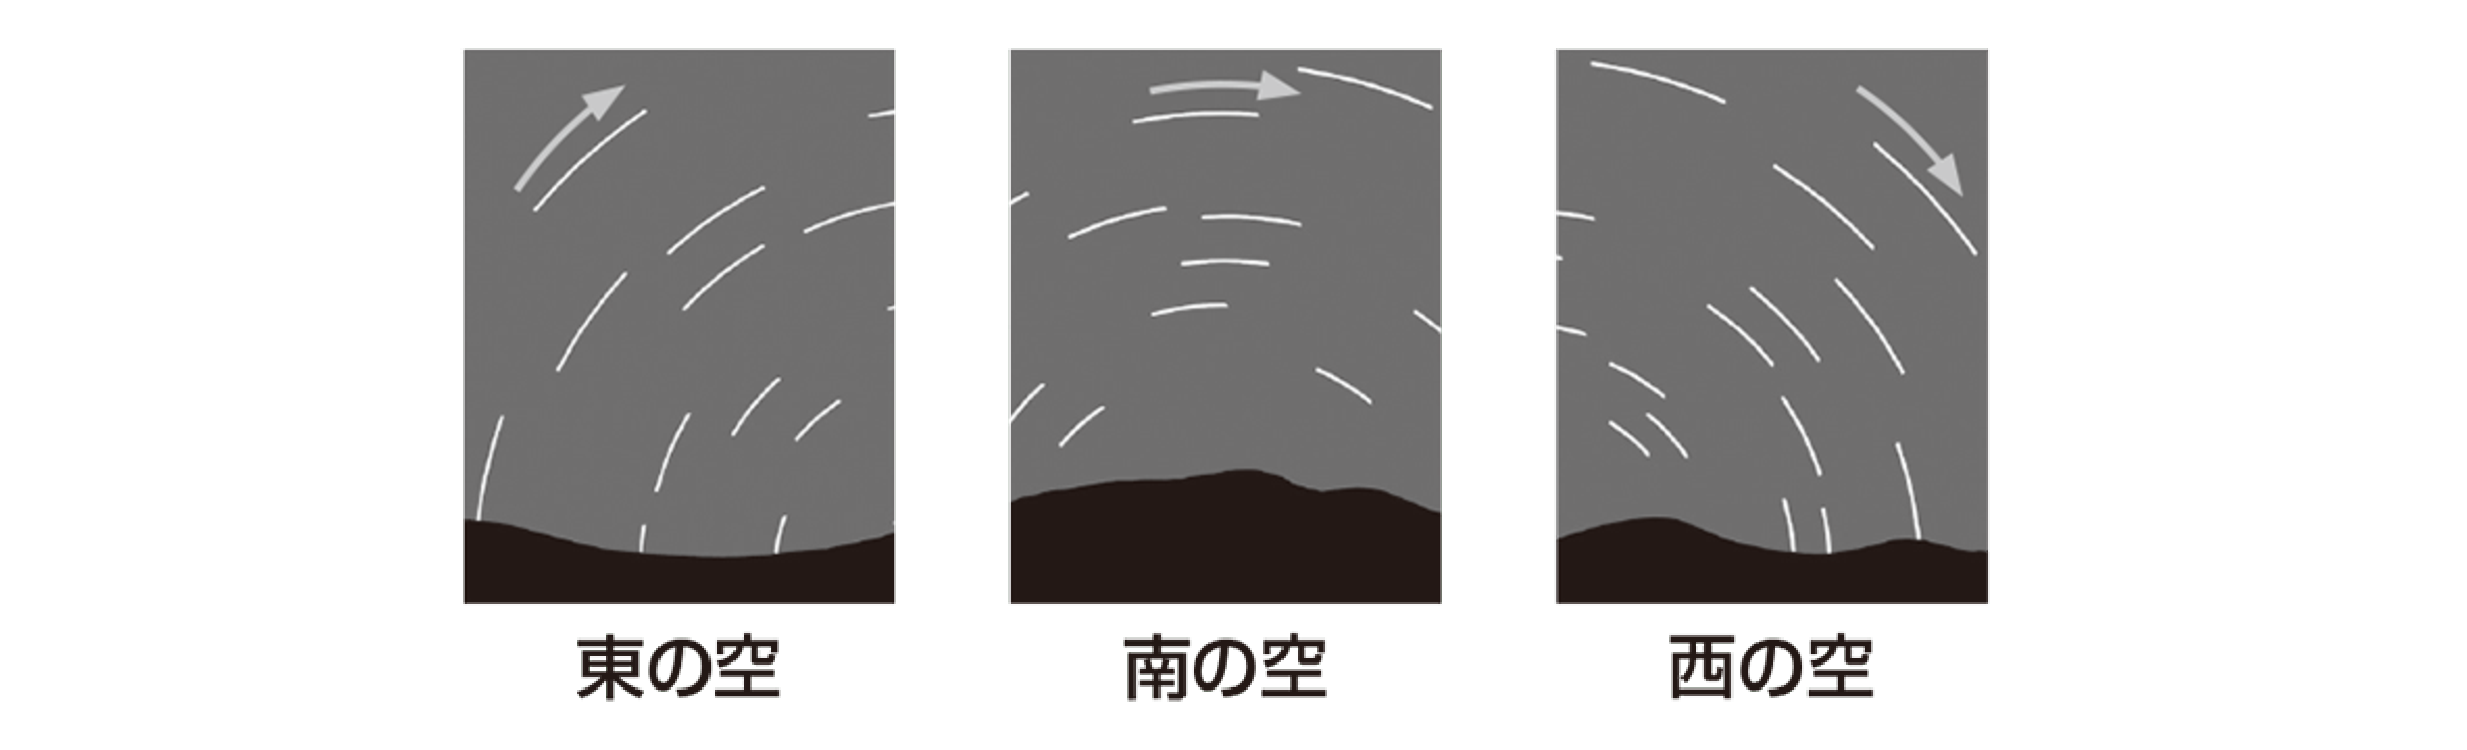
\includegraphics[height=5cm]{science_figure/seiza_minami.pdf}
		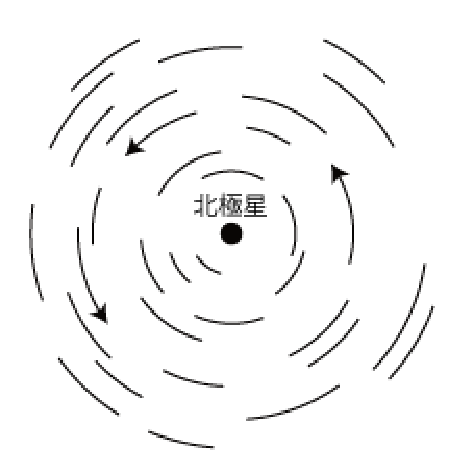
\includegraphics[height=5cm]{science_figure/seiza_kita.pdf}
	}
\end{itembox}

\end{document}
